\chapter{Datasets}
\label{chap:datasets}

\section{QA}
\todo{Standford Question Answering Dataset (SQuAD), 100k questions posed by crowdworkers based on wikipedia atricles. bAbI. Farbes.}
\section{Dialogue Systems}
\todo{Twitter conversation Triple Dataset (BLEU). Ubuntu Dialogue dataset.}

\section{Evaluation}
\todo{As a beginner, it is difficult to get started at evaluating a model, and moreover, there are no simple answer about what metric to use. Here we need to find the tools to mainly evaluate QA systems and sequence to sequence generated texts.}

\section{QA}
\todo{QA could provide quantifiable tasks to test a system reasoning.}
\paragraph{2016 Ubuntu Dialogue Corpus. 1 Million multi turn dialogues, 7 million utterances and 100 million words.}
\todo{}
\paragraph{SQuAD}
\todo{2018 SQuAD 2.0 over 2016 1.0 includes 50'000 unanswerable questions similar to answerable ones (adversarially). It's a closed dataset that gives the answers to question to a given context. It focuses on extreme confusing questions. However it doesn't contain questions that require common sense or reasoning. Wikipedia based. Keeps track of the previous interactions. Yes/No answers accepted for abstractions. }
\paragraph{TriviaQA}
\todo{2017. 650k question-answer-evidence triples.}
\paragraph{MS MARCO}
\todo{2016. (Machine Reading Comprehension). Has been used to evaluate generative models from Seq2Seq, Memory Networks, and Disciminative models. Uses Real and anonymized user queries from Bing. Context is given by a real web documents. All answers are human generated. Subsets are multiples anwsers or no as. All queries are tagged with segment informations. }
\paragraph{CoQa}
\todo{2019. Wikipedia based and 6 other domains. Keeps track of the previous interactions. Yes/No answers accepted. Allows crowd to add an }
\paragraph{QuAC}
\todo{2018. Focus on missing information. Wikipedia based. Keeps track of the previous interactions. Yes/No answers accepted for abstract questions. They doesn't allow the crowd to see the context before formulating the question.}

\paragraph{A Qualitative Comparision of CoQA, SquAD 2.0 and QuAC, 2019}
\todo{Test of the Unanswerable questions, multi-turn interactions, and abstractive answers. Responses are produced by crowd about a paragraph of text, and required to provide a span of text validating their answers. None of the datasets are providing }

\paragraph{Natural Questions Corpus}
\todo{2019. Google dataset (Natural Questions: a Benchmark for Question Answering Research). It's goal is to provide an appropriate training and testing set for QA. It pairs real user queries to what they self call high quality annotations of answers in documents. It also provide metrics to evaluate the performances. Mainly based on a wikipedia, it provides the page, a long and a short answer, and additionally statistics.}

\paragraph{GLUE}
\todo{2019. Banchmarking tool based on existing datasets, which 4 of them are private.}


\begin{figure}[ht!]
    \centering
    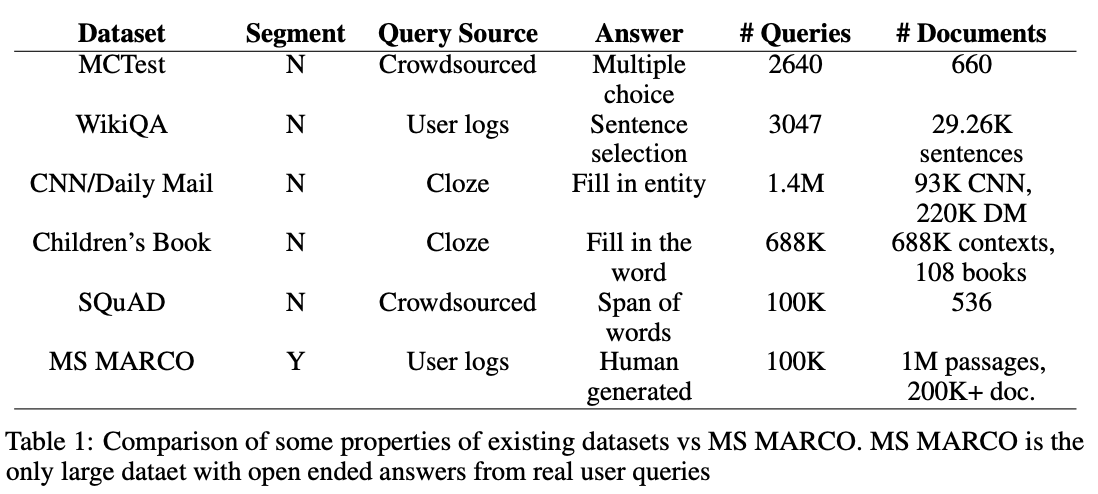
\includegraphics[width=\textwidth,keepaspectratio=true]
    {98-figures/tmp-compare-mas-marco}
    \caption{TMP comparative table took from MS-MARCO}
    \label{fig:tmp-compare-mas-marco}
\end{figure}



